\documentclass{article}
\usepackage{graphicx}
\usepackage{hyperref}
\usepackage{xeCJK}
\usepackage{fontspec}
\usepackage{geometry}
\geometry{margin=1in}

\setlength{\parskip}{1em} % Add spacing between paragraphs
\setlength{\parindent}{0pt} % Disable paragraph indentation

\title{\textbf{Write Out Loud:\\A Multimodal Approach to Learning Chinese Characters}}
\author{Junru Ren \texttt{<junruren@mit.edu>} \\ Freya Tan \texttt{<freya117@mit.edu>}}
\date{\today}

\begin{document}

\maketitle

\fbox{%
\begin{minipage}{\dimexpr\textwidth\fboxsep\fboxrule}
    \section*{Context:}
    The project was only ideated the night before Design Studio on April 8, 2025 as our original
    project idea (``City Moments'') were deemed infeasible for the scope of this class project. We had to quickly brainstorm
    a new idea so as this ``updated'' proposal is due, we are still actively putting together important information such as
    software libraries.
\end{minipage}%
}

\section*{Problem Statement and Basic Idea}
Learning Chinese characters is challenging due to the complexity of multiple aspects including stroke order, pronunciation, and visual recognition. Traditional learning methods often fail to provide immediate multisensory feedback that could enhance memorization and calligraphic skills.

\begin{figure}[h]
    \centering
    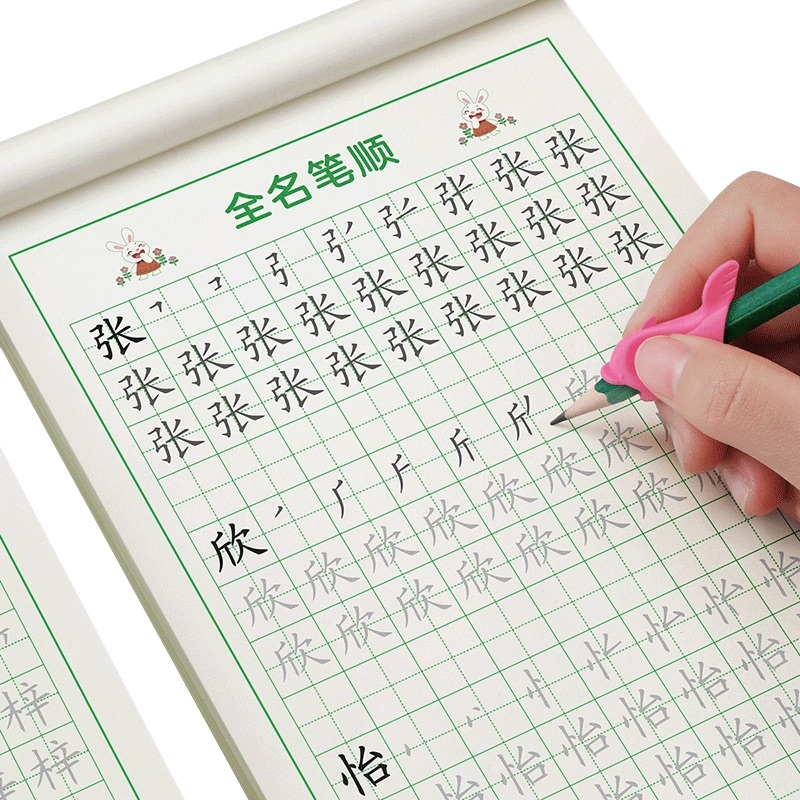
\includegraphics[width=0.25\columnwidth]{Assets/traditional_method.jpeg}
    \caption{Copybook (``字帖''): a traditional paper-based learning tool}
\end{figure}

Our solution, ``Write Out Loud," is a multimodal educational tool designed to aid learners of Chinese characters by
integrating handwriting and speech modalities. As learners trace each character's strokes, they are required to
simultaneously vocalize stroke names. The system provides real-time feedback to evaluate:
\begin{enumerate}
    \item How accurately each stroke was traced?
    \item Was stroke order followed?
    \item How timely and accurately was the stroke name vocalized?
\end{enumerate}
So that the learner masters the character through a combination of visual, auditory, and kinesthetic learning
modalities.

\subsection*{Goal}
The goal of this app is to improve \textbf{handwriting} of Chinese characters but not pronunciation (which can be a
future feature addition).  The deliberate vocalization of each stroke is meant to reinforce the learning of stroke
order. As such, the app will not evaluate the pronunciation of each stroke name as long as the learner vocalizes the
correct stroke name. 

\subsection*{Concrete Example Scenario}

A learner uses ``Write Out Loud" on an iPad with a compatible writing stylus (e.g., Apple Pencile).

When the learner selects a character, the app displays, on the non-writing half of the screen
\footnote{We strive to use ``the writing half'' and ``the non-writing half'' to avoid being biased towards the right-handed or left-handed population. For for illustrative purpose, we assume that the left side of the screen is the non-writing half where necessary information is displayed.}
, that character overlaid with an animation showing how strokes are to be traced through.

On the writing half of the screen, the same character is displayed in less saturated grey color for the learner to trace
through using their stylus.

\begin{figure}[h]
    \centering
    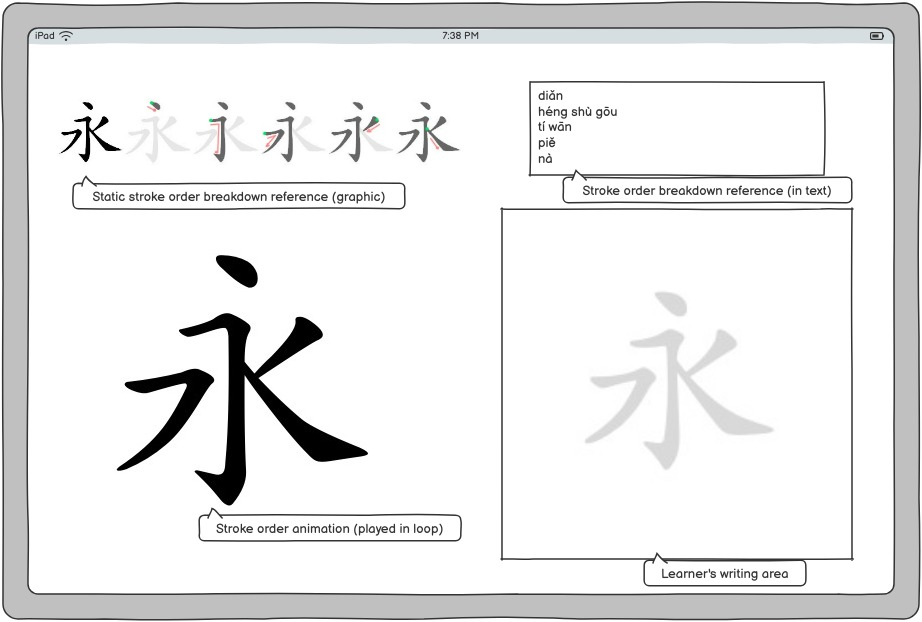
\includegraphics[width=0.75\columnwidth]{Assets/App_Mockup.jpg}
    \caption{Mockup of app's writing GUI}
\end{figure}

The learner traces the first stroke, vocalizing its stroke name (e.g., ``shù"). The app simultaneously captures the temporal and spatial handwriting input and timestamps the audio input. And so on. Once the character is detected to be fully traced. The app then assesses if the learner vocalized the correct stroke name concurrently with the stroke tracing. Feedback and a performance score are displayed after completing all strokes of the character, guiding learners to improve in subsequent attempts.

\section*{Relevant Published Background}

Multisensory learning, which engages multiple senses such as visual, auditory, kinesthetic, and tactile modalities, has
been extensively studied for its benefits in enhancing educational outcomes. Studies indicate that this approach
improves memory retention by engaging multiple sensory pathways, leading to stronger neural connections
\footnote{Okray, Z., Jacob, P.F., Stern, C. et al. Multisensory learning binds neurons into a cross-modal memory engram. Nature 617, 777–784 (2023). \href{https://doi.org/10.1038/s41586-023-06013-8}{https://doi.org/10.1038/s41586-023-06013-8}}. Engaging multiple senses caters to diverse learning styles, facilitating better understanding of
complex concepts.


\section*{Planned Implementation and Basic Architecture}
Our application will run on iPadOS, utilizing Apple Pencil for precise handwriting input and built-in microphone capabilities for capturing vocalizations.

\textbf{System Components:}
\begin{itemize}
    \item \textbf{Pen Stroke Input Module}: Captures temporal and spatial data of stroke tracing.
    \item \textbf{Speech Input Module}: Records timestamped audio of stroke pronunciation.
    \item \textbf{Trace Analyzer}: Scores tracing accuracy based on predefined stroke patterns.
    \item \textbf{Speech Recognition Module}: Evaluates the correctness of stroke names vocalized by the learner.
    \item \textbf{Concurrency Analyzer}: Assesses the simultaneity of speech and handwriting inputs.
\end{itemize}

\begin{figure}[h!]
\centering
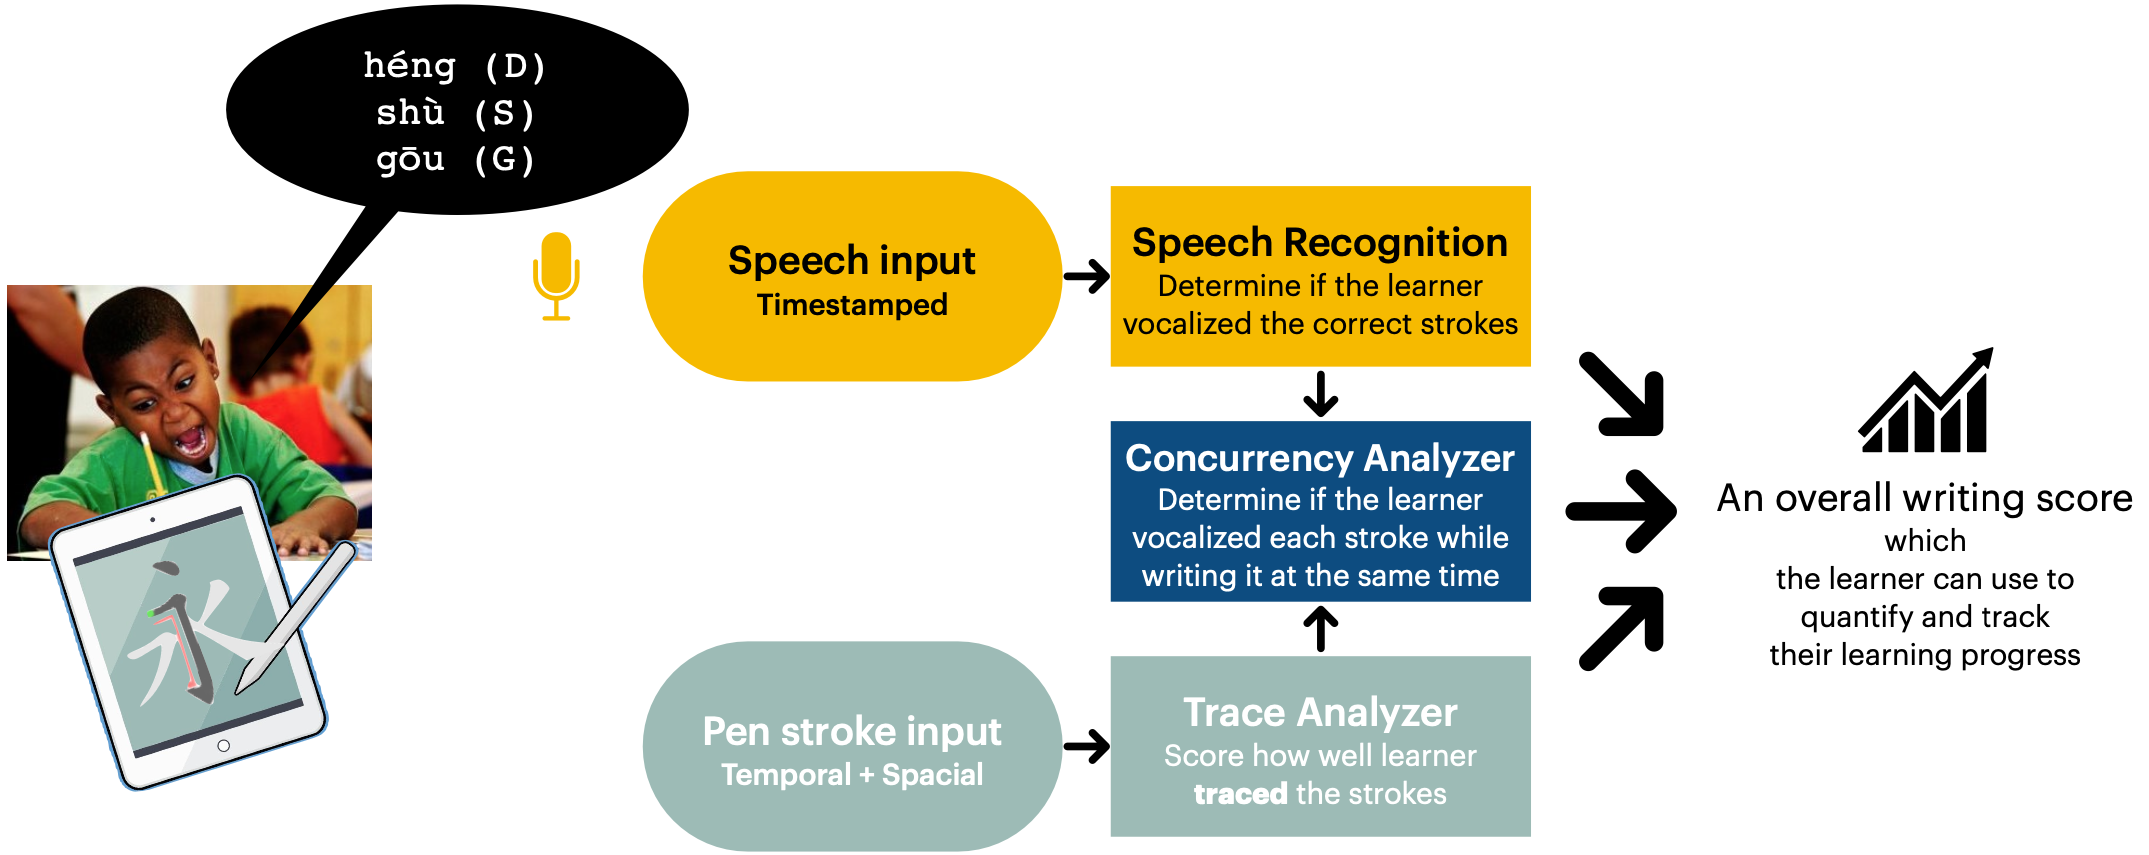
\includegraphics[width=0.8\textwidth]{Assets/SystemDiagram.png}
\caption{System Architecture Diagram of ``Write Out Loud"}
\label{fig:system}
\end{figure}

\section*{Required Resources}
\begin{itemize}
    \item iPad device with Apple Pencil
    \item Speech recognition software (built-in iOS Speech Framework)\footnote{Apple's \texttt{SFSpeechRecognizer} library: \href{https://developer.apple.com/documentation/speech}{https://developer.apple.com/documentation/speech}}
    \item Handwriting recognition and stroke analysis software (custom-built)\footnote{
    Apple's \texttt{PencilKit} library: \href{https://developer.apple.com/documentation/pencilkit}{https://developer.apple.com/documentation/pencilkit}}
    \item A small hand-curated\footnote{In a class project scope, we decided to just manually create data for few character as our focus in on the interaction of learning a character but not production-ready coverage.} Chinese character dataset that includes the following for each character:
    \begin{itemize}
        \item Visual representation of the entire character
        \item Visual representation of the entire character in grey for trace over
        \item Animation of the stroke order
        \item Stroke order (graphic and textual)
        \item Broken down stroke coordinates within the writing pane
    \end{itemize}
\end{itemize}

\section*{Experimental Evaluation}
We will first evaluate the system using a baseline character, such as ``口," which involves simple, well-defined strokes. Participants will complete tasks of writing and vocalizing characters, with performance metrics captured across both modalities. Metrics on the learner include accuracy of stroke tracing, correctness of vocalizations, and the timing alignment between writing and speaking. For the app itself, we will measure learner satisfaction and subjective ease of use. We also plan to invite a small group of people who doesn't know Chinese to try the fined app and then test whether they could write the same set of characters on paper later after using the app.

\textbf{Evaluation Metrics:}
\begin{itemize}
    \item Accuracy of stroke tracing (shape, order, and orientation)
    \item Correctness and clarity of vocalized stroke names
    \item Temporal alignment between writing and vocalizing
    \item Feedback delivery effectiveness (e.g., text/audio corrections)
    \item Usability feedback through post-task surveys and interviews
\end{itemize}

% \textbf{Highlight:} Your presentation did not specify detailed evaluation metrics, how performance will be quantitatively measured, nor how you will assess usability qualitatively. You should elaborate on these metrics clearly.

\section*{Staged Development Plan}

\begin{table}[htbp]
    \centering
    \begin{tabular}{|c|c|p{0.6\textwidth}|}
        \hline
        \textbf{Version} & \textbf{Deadline} & \textbf{Description} \\
        \hline
        V-0 & April 13 & Set up the iPadOS development environment and write a dummy iPadOS app via XCode. \\
        \hline
        V-1 & April 27 & Implement basic functionality to capture handwriting and vocalization for a simple set of characters, providing accuracy feedback. \\
        \hline
        V-2 & May 2 & Expand character set and refine feedback mechanisms. \\
        \hline
        V-3 & May 5 & Enhance user interface and integrate adaptive learning features based on user performance. \\
        \hline
    \end{tabular}
    \caption{Staged Development Plan}
    \label{tab:dev_plan}
\end{table}
\end{document}
